% Written by Michaël Museux

\subsubsection*{Le Multijoueur}

Pour pouvoir organiser une partie multijoueur, nous avons décidé d'utiliser l'API intégrée à Godot.
Pour cela, il nous faut un serveur, ici l'hôte, ainsi que les joueurs qui rejoignent sa partie appelés les clients,
En premier temps, l'hôte doit choisir quel port il souhaite utiliser pour sa partie, puis les joueurs doivent accéder à l'adresse de l'hôte, ainsi que le port précédemment choisi (cf Figure \ref{fig:gameplay1} et \ref*{fig:gameplay2}).

\begin{figure}[H]
    \centering
    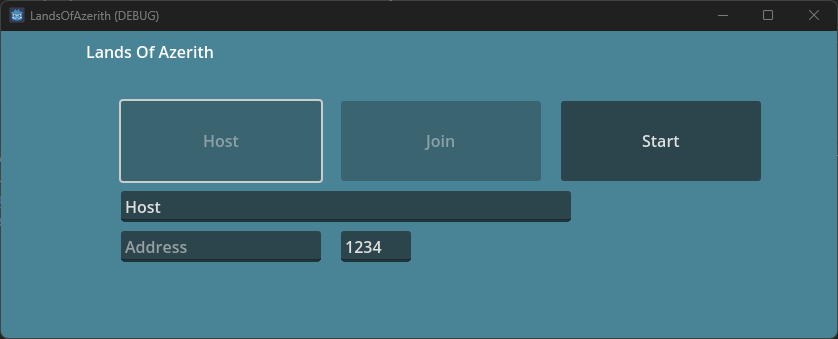
\includegraphics[width=0.8\textwidth]{2.game/assets/gameplay1.png}
    \caption{L'hôte clique sur "Host" et choisi le port 1234}
    \label{fig:gameplay1}
\end{figure}

\begin{figure}[H]
    \centering
    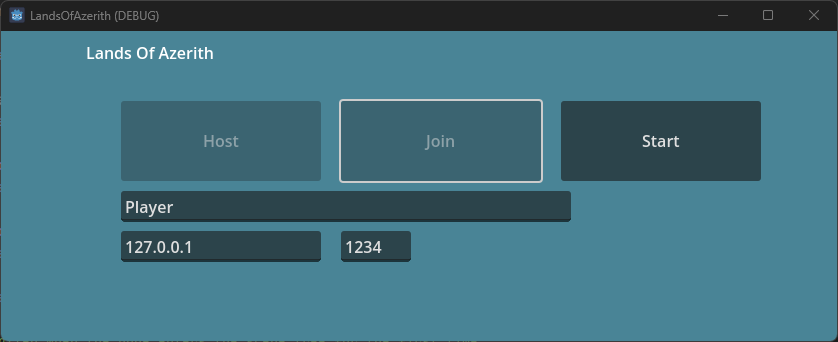
\includegraphics[width=0.8\textwidth]{2.game/assets/gameplay2.png}
    \caption{Le client clique sur "Join" et choisi le port 1234 à l'adresse 127.0.0.1.}
    \label{fig:gameplay2}
\end{figure}

Il est possible de jouer avec un nombre infini de joueurs, mais nous avons établi un maximum de 8, limite que nous utiliserons lors de la conception du reste du jeu.
\\

Maintenant que la connexion est établie entre les différents joueurs, il nous faut synchroniser leurs informations entre eux, tout en faisant attention à ne pas trop partager d'informations inutiles, pour limiter l'utilisation de bande passante.
Par exemple, la synchronisation des positions de chacun entre tous les joueurs est importante, mais la position de la caméra d'un joueur n'est nécessaire qu'en local (c.f. Figures \ref*{fig:gameplay3} et \ref*{fig:gameplay4}).

\begin{figure}[H]
    \centering
    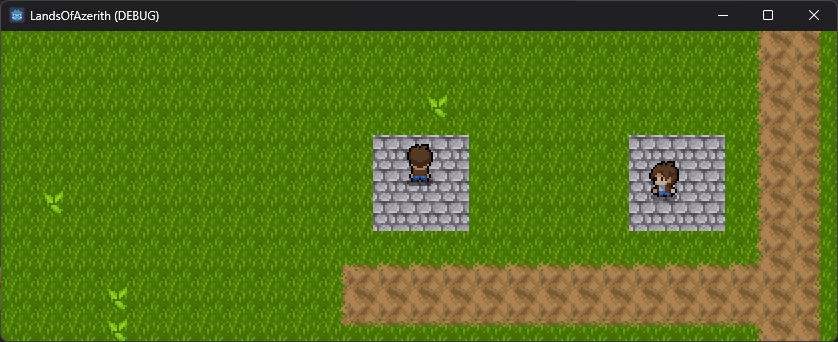
\includegraphics[width=0.8\textwidth]{2.game/assets/gameplay3.png}
    \caption{Le joueur 1 regarde vers le haut sur le carré de gauche avec sa caméra centré sur lui, le joueur 2 est à droite.}
    \label{fig:gameplay3}
\end{figure}

\begin{figure}[H]
    \centering
    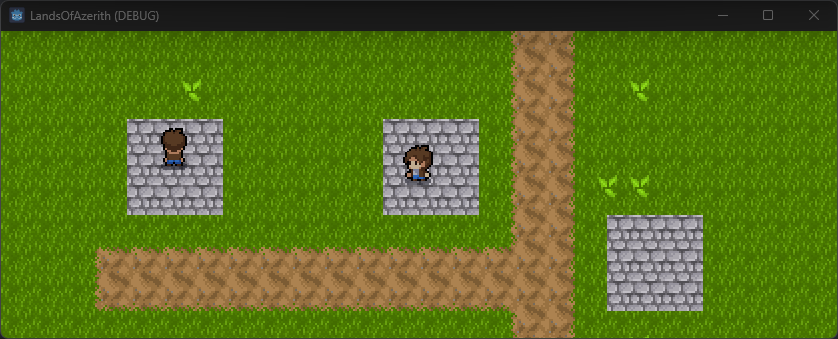
\includegraphics[width=0.8\textwidth]{2.game/assets/gameplay4.png}
    \caption{Le joueur 2 regarde vers la gauche sur le carré de droite avec sa caméra centré sur lui, le joueur 1 est à gauche.}
    \label{fig:gameplay4}
\end{figure}


\subsubsection*{Déplacement et comportement des PNJ}

Au cours des aventures de nos joueurs, ceux-ci rencontreront des monstres et animaux, passifs ou agressifs.
Il nous faut donc implémenter ces différents comportements.
Pour commencer, chaque PNJ est dans l'état “\textit{Wander}”, c'est-à-dire qu'il va soit trouver un endroit aléatoire où aller, soit rester sur place (c.f. Figure 5)

\begin{figure}[H]
    \centering
    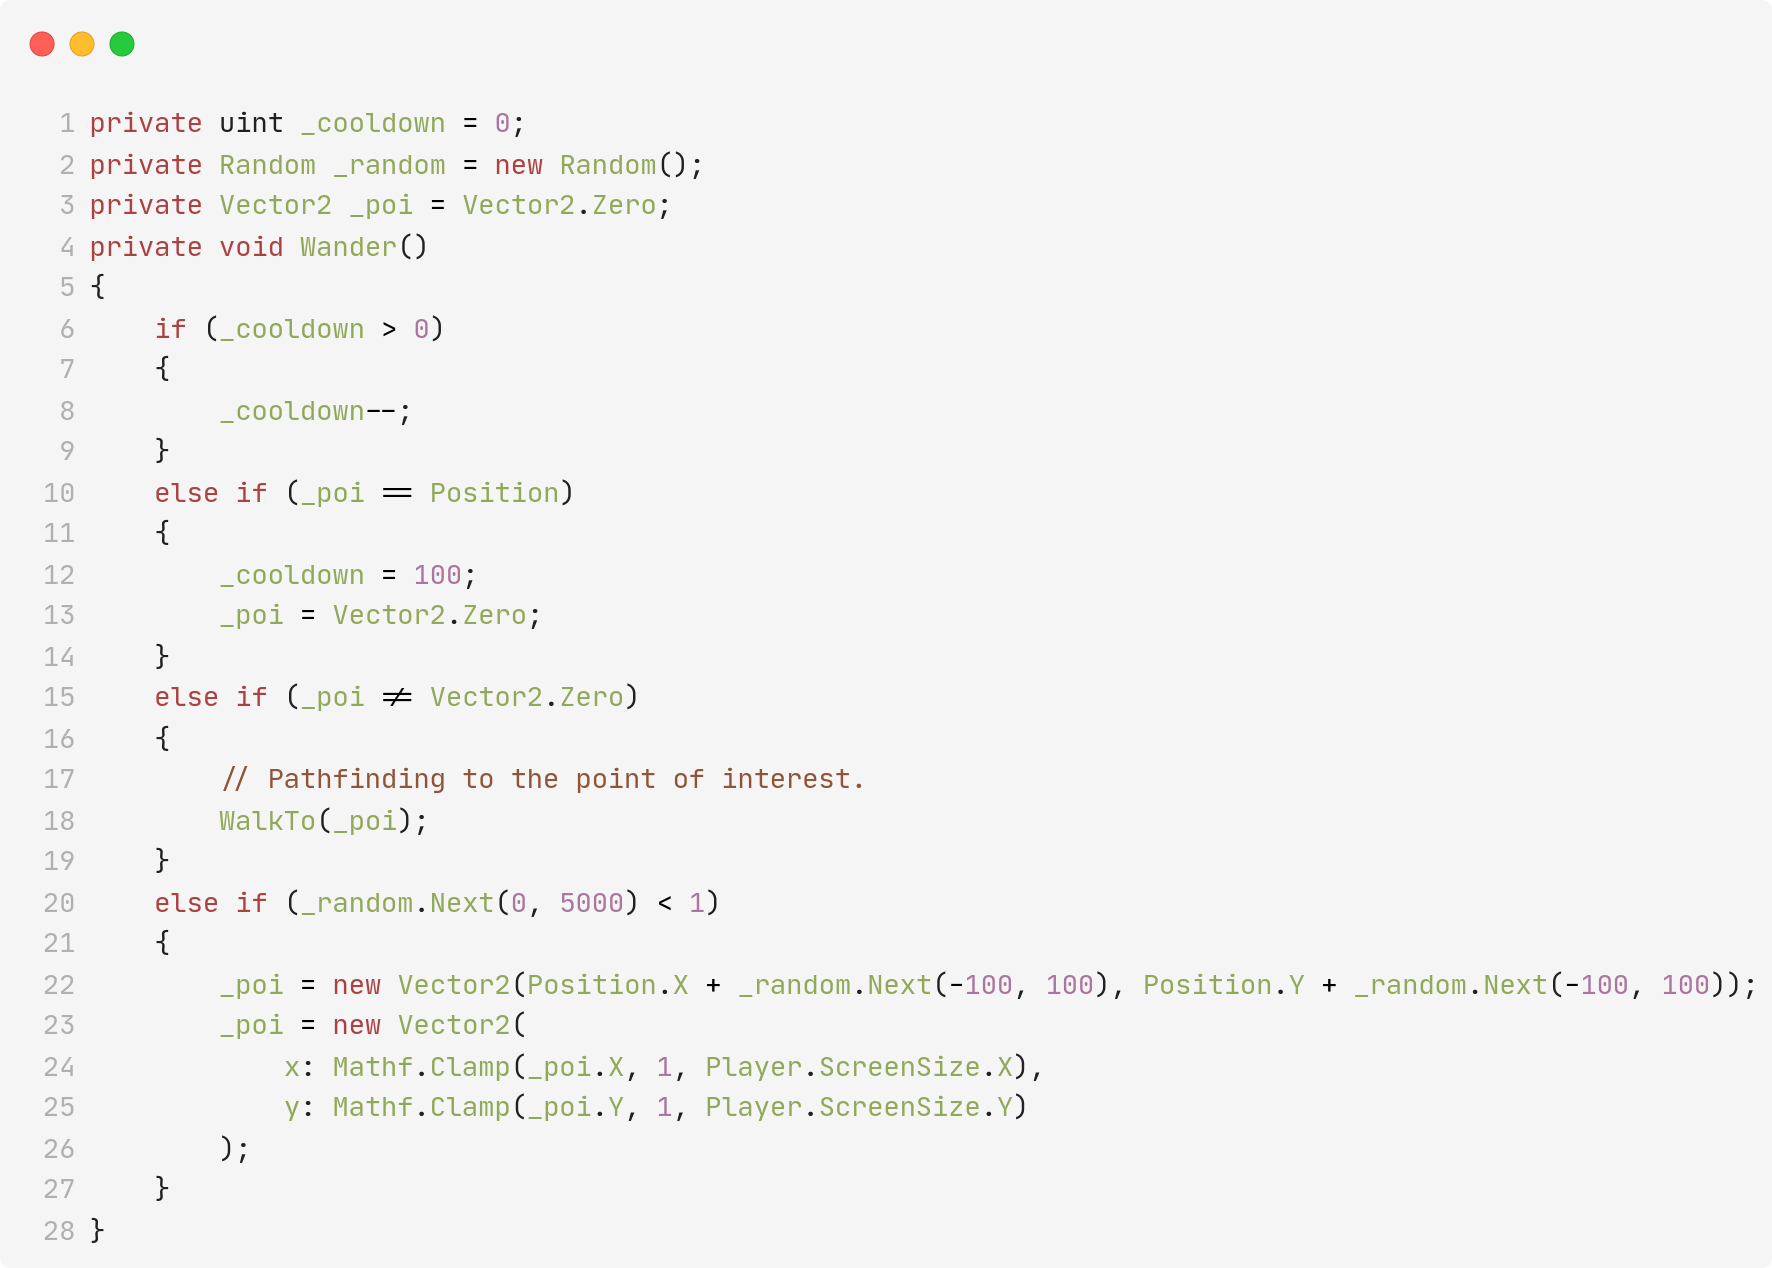
\includegraphics[width=1.0\textwidth]{2.game/assets/gameplay5.png}
    \caption{Code C\# décrivant le comportement durant l'état “\textit{Wander}”}
    \label{fig:gameplay5}
\end{figure}

Ensuite, le comportement d'une créature va brancher en quatre catégories distinctes :

- Le PNJ Agressif va attaquer le joueur lorsqu'il est à proximité

- Le PNJ Neutre ne va pas réagir au joueur lorsqu'il est à proximité, mais va répondre à ses attaques

- Le PNJ Passif ne va pas réagir au joueur lorsqu'il est à proximité, mais va fuir s'il est attaqué

- Le PNJ Peureux va fuir lorsqu'il est à proximité du joueur.
\\

\begin{figure}[H]
    \centering
    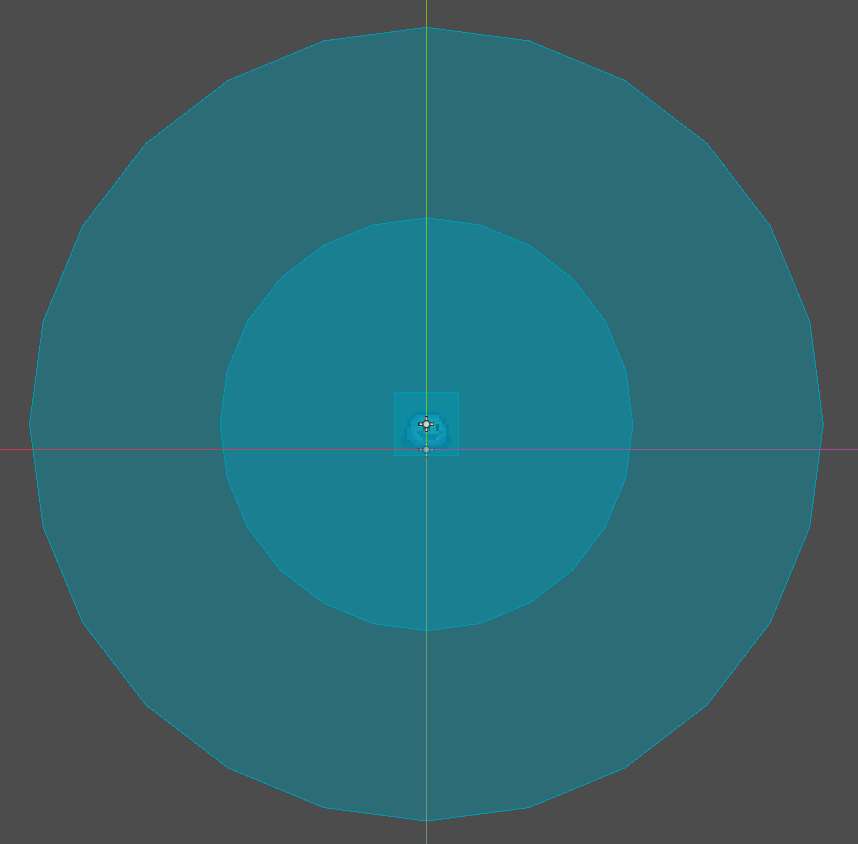
\includegraphics[width=0.8\textwidth]{2.game/assets/gameplay6.png}
    \caption{PNJ Agressif, avec ses zones d'\textit{aggro} et de \textit{déaggro}}
    \label{fig:gameplay6}
\end{figure}

Pour la détection du joueur, nous allons utiliser la fonctionnalité des signaux de Godot, et initier deux zones de détection circulaire autour de chaque monstre.
La première servira à détecter lorsque le joueur rentre dans cette zone (zone d'aggro), et la deuxième, un peu plus grande, qui détectera la sortie du joueur de cette zone (zone de déaggro), et qui repassera le PNJ dans l'état \textit{Wander}.
On ne veut pas qu'il fuit ou qu'il attaque le joueur pendant toute la durée de la partie (c.f. Figure \ref*{fig:gameplay6}).


\subsubsection*{Les quêtes, les classes, l'inventaire et la sauvegarde}

Nous nous sommes concentrés sur l'implémentation du multijoueur ainsi que d'une partie de l'IA des PNJ, car nous pensons que pour pouvoir intégrer plus de contenu, il nous faut une base solide, ainsi qu'une bonne compréhension du fonctionnement de jeu en multijoueur.
\\

Nous avons donc prévu à la suite de cette soutenance de terminer le comportement des PNJ, puis de poursuivre sur le fonctionnement de la sauvegarde de données, ainsi que les classes de joueurs, les quêtes et l'inventaire.
